\documentclass{standalone}
\usepackage{tikz}

\begin{document}
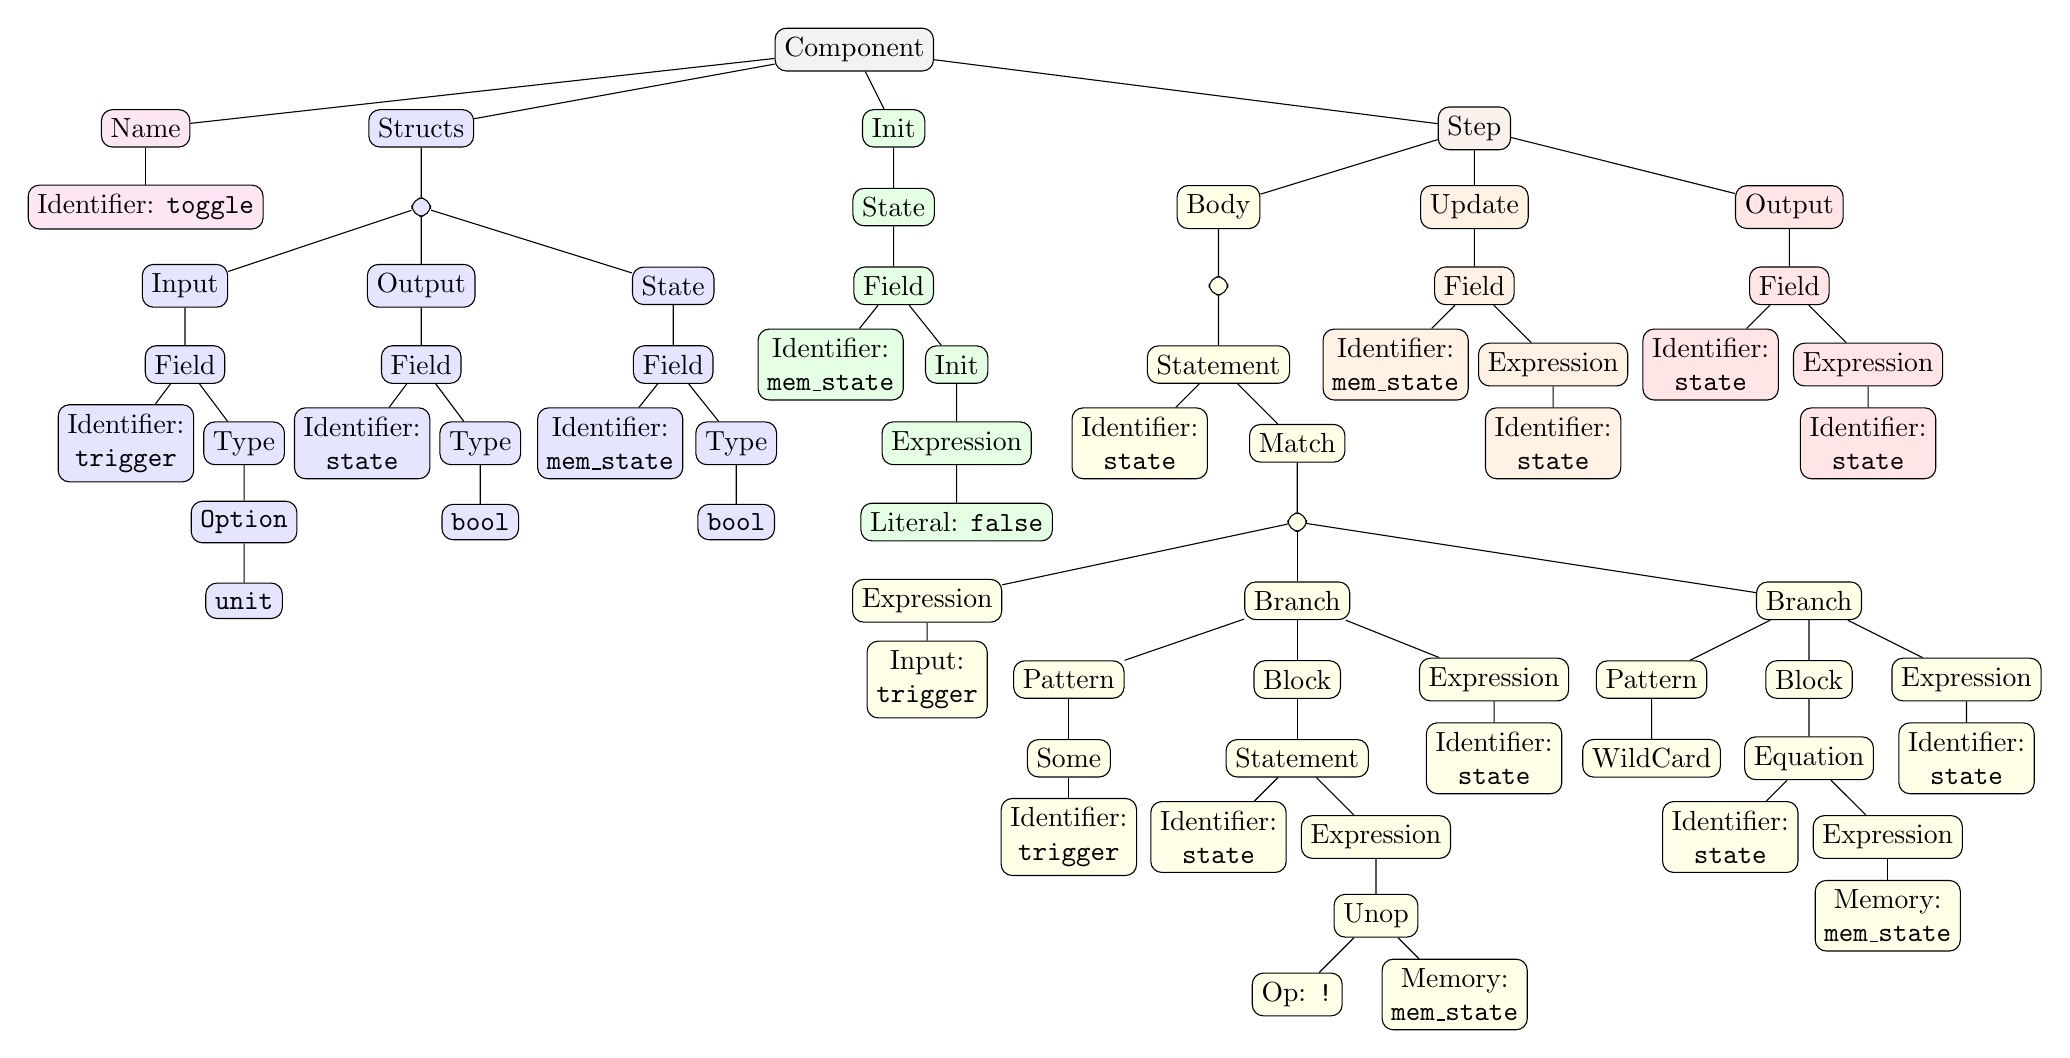
\begin{tikzpicture}[
                level distance=1cm, sibling distance=3cm,
                treenode/.style = {rectangle, rounded corners, fill=gray!10, draw, align=center}
        ]
        \node[treenode] {Component}
        child [sibling distance=6cm] { node[treenode, fill=magenta!10] {Name} child { node[treenode, fill=magenta!10] {Identifier: \texttt{toggle}} } }
        child [sibling distance=11cm] { node[treenode, fill=blue!10] {Structs}
                        child { node[treenode, fill=blue!10] {}
                                        child [sibling distance=3cm] { node[treenode, fill=blue!10] {Input}
                                                        child [sibling distance=1.5cm] { node[treenode, fill=blue!10] {Field}
                                                                        child { node[treenode, fill=blue!10] {Identifier:\\\texttt{trigger}} }
                                                                        child { node[treenode, fill=blue!10] {Type} child { node[treenode, fill=blue!10] {\texttt{Option}} child { node[treenode, fill=blue!10] {\texttt{unit}} }  }  }
                                                                }
                                                }
                                        child [sibling distance=3cm] { node[treenode, fill=blue!10] {Output}
                                                        child [sibling distance=1.5cm] { node[treenode, fill=blue!10] {Field}
                                                                        child { node[treenode, fill=blue!10] {Identifier:\\\texttt{state}} }
                                                                        child { node[treenode, fill=blue!10] {Type} child { node[treenode, fill=blue!10] {\texttt{bool}} }  }
                                                                }
                                                }
                                        child [sibling distance=3.2cm] { node[treenode, fill=blue!10] {State}
                                                        child [sibling distance=1.6cm] { node[treenode, fill=blue!10] {Field}
                                                                        child { node[treenode, fill=blue!10] {Identifier:\\\texttt{mem\_state}} }
                                                                        child { node[treenode, fill=blue!10] {Type} child { node[treenode, fill=blue!10] {\texttt{bool}} }  }
                                                                }
                                                }
                                }
                }
        child [sibling distance=1cm] { node[treenode, fill=green!10] {Init}
                        child [sibling distance=3.2cm] { node[treenode, fill=green!10] {State}
                                        child [sibling distance=1.6cm] { node[treenode, fill=green!10] {Field}
                                                        child { node[treenode, fill=green!10] {Identifier:\\\texttt{mem\_state}} }
                                                        child { node[treenode, fill=green!10] {Init} child { node[treenode, fill=green!10] {Expression} child { node[treenode, fill=green!10] {Literal: \texttt{false}} } } }
                                                }
                                }
                }
        child [sibling distance=5.25cm] { node[treenode, fill=brown!10] {Step}
                        child [sibling distance=3.25cm] { node[treenode, fill=yellow!10] {Body}
                                        child { node[treenode, fill=yellow!10] {}
                                                        child { node[treenode, fill=yellow!10] {Statement}
                                                                        child [sibling distance=2cm] { node[treenode, fill=yellow!10] {Identifier:\\\texttt{state}}}
                                                                        child [sibling distance=2cm] { node[treenode, fill=yellow!10] {Match}
                                                                                        child { node[treenode, fill=yellow!10] {}
                                                                                                        child [sibling distance=4.7cm] { node[treenode, fill=yellow!10] {Expression} child { node[treenode, fill=yellow!10] {Input:\\\texttt{trigger}} } }
                                                                                                        child [sibling distance=0cm] { node[treenode, fill=yellow!10] {Branch}
                                                                                                                        child [sibling distance=2.9cm] { node[treenode, fill=yellow!10] {Pattern} child { node[treenode, fill=yellow!10] {Some} child { node[treenode, fill=yellow!10] {Identifier:\\\texttt{trigger}} } } }
                                                                                                                        child [sibling distance=2.9cm] { node[treenode, fill=yellow!10] {Block}
                                                                                                                                        child { node[treenode, fill=yellow!10] {Statement}
                                                                                                                                                        child [sibling distance=2cm] { node[treenode, fill=yellow!10] {Identifier:\\\texttt{state}} }
                                                                                                                                                        child [sibling distance=2cm] { node[treenode, fill=yellow!10] {Expression}
                                                                                                                                                                        child { node[treenode, fill=yellow!10] {Unop}
                                                                                                                                                                                        child { node[treenode, fill=yellow!10] {Op: \texttt{!}} }
                                                                                                                                                                                        child { node[treenode, fill=yellow!10] {Memory:\\\texttt{mem\_state}} }
                                                                                                                                                                                }
                                                                                                                                                                }
                                                                                                                                                }
                                                                                                                                }
                                                                                                                        child [sibling distance=2.5cm] { node[treenode, fill=yellow!10] {Expression} child { node[treenode, fill=yellow!10] {Identifier:\\\texttt{state}} } }
                                                                                                                }
                                                                                                        child [sibling distance=6.5cm] { node[treenode, fill=yellow!10] {Branch}
                                                                                                                        child [sibling distance=2cm] { node[treenode, fill=yellow!10] {Pattern} child [sibling distance=3cm] { node[treenode, fill=yellow!10] {WildCard} } }
                                                                                                                        child [sibling distance=2cm] { node[treenode, fill=yellow!10] {Block}
                                                                                                                                        child [sibling distance=3cm] { node[treenode, fill=yellow!10] {Equation}
                                                                                                                                                        child [sibling distance=2cm] { node[treenode, fill=yellow!10] {Identifier:\\\texttt{state}} }
                                                                                                                                                        child [sibling distance=2cm] { node[treenode, fill=yellow!10] {Expression}
                                                                                                                                                                        child { node[treenode, fill=yellow!10] {Memory:\\\texttt{mem\_state}} }
                                                                                                                                                                }
                                                                                                                                                }
                                                                                                                                }
                                                                                                                        child [sibling distance=2cm] { node[treenode, fill=yellow!10] {Expression} child { node[treenode, fill=yellow!10] {Identifier:\\\texttt{state}} } }
                                                                                                                }
                                                                                                }
                                                                                }
                                                                }
                                                }
                                }
                        child [sibling distance=4cm] { node[treenode, fill=orange!10] {Update}
                                        child [sibling distance=2cm] { node[treenode, fill=orange!10] {Field}
                                                        child { node[treenode, fill=orange!10] {Identifier:\\\texttt{mem\_state}} }
                                                        child { node[treenode, fill=orange!10] {Expression} child { node[treenode, fill=orange!10] {Identifier:\\\texttt{state}} } }
                                                }
                                }
                        child [sibling distance=4cm] { node[treenode, fill=red!10] {Output}
                                        child [sibling distance=2cm] { node[treenode, fill=red!10] {Field}
                                                        child { node[treenode, fill=red!10] {Identifier:\\\texttt{state}} }
                                                        child { node[treenode, fill=red!10] {Expression} child { node[treenode, fill=red!10] {Identifier:\\\texttt{state}} } }
                                                }
                                }
                };
\end{tikzpicture}
\end{document}
